\chapter{Grundlagen}

\section{Extraktion von Entitäten} \label{sec:Grundlagen}
\paragraph{}
%Was sind die Entitäten - kurze Einleitung. Wie genau können die Entitäten aus einem Text extrahiert werden? Welche Einsätze gibt es? Wofür kann man Entitäten verwenden?
Vijay Krishnan hat in seiner Arbeit\cite{Vijay/Vignesh:05} die Extraktion von Entitäten als Suche nach atomaren Elementen im Text und ihre Zuordnung bestimmten vordefinierten Klassen wie Person, Organisation, geographische Lokation usw. definiert. Zum Beispiel betrachten wir folgenden Text aus Wikipedia: ,,Seit dem 1. Januar 2014 ist Bill de Blasio neuer Bürgermeister von New York.``. Dabei soll das Framework, das die Entitäten aus dem Text extrahiert, die Entität \textit{Bill de Blasio} als eine Person erkennen, die Entität \textit{New York} als ein geographisches Objekt, und \textit{1. Januar 2014} als ein Datum.

\paragraph{}
Es stellt sich die Frage, wie genau die Entitäten für die Benutzerunterstützung bei der Suche eingesetzt werden können. Wenn die einzige Informationen, die dem Benutzer zur Verfügung stehen würde, nur der Name, die Klasse und Position der Entität innerhalb des Textes wären, wären Entitäten kaum verwendbar. Aber wenn jeder Entität eine Menge von Eigenschaften (wie Geburtsdatum für eine Person) und Verbindungen zu anderen Entitäten (Z.b. Geburtsort einer Person könnte ein Link auf eine geografische Entität sein) zugeordnet wird, könnte der Benutzer theoretisch die aus der Entität gewonnene Informationen für Präzisierung der Suchanfrage verwenden.

\paragraph{}
Aber wie könnten die Entitäten aus einem natürlichsprachlichen Text extrahiert werden? Die einfachste Möglichkeit wäre der Einsatz von ,,fest definierten`` Regeln, die dann auf den ganzen Text angewendet werden, und entscheiden, ob das nächste Wort eine Entität ist oder nicht. Dieser Einsatz soll in dieser Arbeit aber nicht eingesetzt werden, da er folgende Nachteile\cite{baluja2000applying} hat:
\begin{enumerate}
\item So ein ,,festes`` System ist nicht in der Lage, Änderungen automatisch zu 'erlernen' und muss für jede Änderung neu angepasst/programmiert werden.
\item Derartige ,,feste`` Systeme neigen dazu, mit der Zeit sehr komplex zu werden, und ab irgendeinem Zeitpunkt wird die Anpassung von Regeln unmöglich beziehungsweise mit einem großen technischem Aufwand verbunden sein.
\item Solche Systeme können nicht wirklich gut mit den fehlerhaften Daten wie Schreibfehler arbeiten, was im Fall von Websuche sehr oft auftreten kann.
\end{enumerate}  
Der einzige Vorteil von solchen festen Systemen ist dass die für sehr kleine Domäne eventuell gut funktionieren können, was allerdings für Websuche nicht ausreichend ist.

Aber welche Methode ist für die Extraktion von Entitäten passend? Wie erwähnt, gehört jede Entität irgendeiner Klasse. Deswegen kann man die Extraktion von Entitäten als Klassifikationsaufgabe definieren, und die Methoden des maschinellen Lernens, die man für die Klassifizierung anwendet, einsetzen, wie es z.B. in der Arbeit von William Cohen\cite{cohen2004exploiting} beschrieben wurde. In dieser Arbeit werden drei verschiedene Einsätze verglichen und eingesetzt: \textbf{Conditional Random Field}, \textbf{Support Vector Machines} und \textbf{Maximum Entropy}.

\subsection{Features}
\paragraph{}
Wie für jede andere Klassifizierungsaufgabe müssen für die Extraktion von Entitäten die Parameter definiert werden, die jedes zu klassifizierendes Objekt beschreiben. Im Fall von Extraktion von Entitäten  heißt das, dass jedem Wort ein Vektor von Eigenschaften zugeordnet werden muss. Nadeau\cite{nadeau2007survey} hat die Eigenschaften, die ein Wort haben kann, in drei Gruppen geteilt:

\begin{itemize}
\item Boolesche Eigenschaften wie ,,Ob das Wort groß geschrieben wird``.
\item Numerische Eigenschaften wie die Länge des Wortes.
\item Nominale Eigenschaften wie Präfix oder Suffix.
\end{itemize}
Zusätzlich dazu wurde von Hai\cite{chieu2002named} die Verteilung in lokale und globale Eigenschaften vorgeschlagen:

\begin{enumerate}
\item Globale Eigenschaften:
\begin{enumerate}
\item Personenpräfixe für bestimmtes Wort in anderen Sätzen des Dokumentes: z.B. wenn wir im Text zuerst die Tokens ,,Frau Sony`` treffen, und dann einfach ,,Sony``, dann soll angenommen werden, dass ,,Sony`` eine Entität der Klasse ,,Person`` ist.
\item Abkürzungen: wenn in einem Satz mehr Wörter nacheinander groß geschrieben werden, wie z.B. ,,Deutsche Demokratische Republik``, dann wird in dem Text nach entsprechender Abkürzung gesucht: ,,DDR``, und wenn Abkürzung eine Entität ist, können auch alle entsprechende Tokens als eine Entität markiert werden.
\end{enumerate}
\item Lokale Eigenschaften:
\begin{enumerate}
\item Ob das Wort groß geschrieben wird.
\item Ob vorheriges oder nächstes Wort großgeschrieben wird.
\item Ob alle Zeichen im Wort großgeschrieben werden.
\item Ob es ein Punkt am Ende des Wortes steht.
\item Ob das Wort Zahlen beinhaltet, und falls ja, wie viel.
\item Ob das Wort das Prozent- oder Dollarzeichen beinhaltet.
\item Bestimmte Hilfswörter (wie ,,Frau`` oder ,,GmbH``), die entweder vor oder nach dem Wort, das untersucht werden muss, stehen.
\item Ob das Wort nur aus Zahlen besteht.
\item POS-Tag des Wortes (ob das Wort ein Substantiv oder ein Verb ist)
\item POS-Tags der Wörter, die vor dem ausgewählten Wort stehen.
\end{enumerate}
\end{enumerate}
Dabei beschreiben lokale Features die Eigenschaften, die nur die Informationen, die aus dem Wort selbst und aus den benachbarten Wörtern in demselben Satz gewonnen werden können, brauchen. Globale Eigenschaften benutzen dagegen auch die Vorkommnisse vom Wort im ganzen Dokument.

Das oben genannte Features werden ,,supervised Features`` genannt, weil die von einem Mensch bestimmt wurden. Zusätzlich dazu wird in der Arbeit von Turian\cite{turian2010word} der Einsatz von sogenannten ,,unsupervised Features`` vorgeschlagen, die während des Lernvorganges berechnet werden. Es wird in der zitierten Arbeit zwischen folgenden Gruppen von ,,unsupervised Features`` unterschieden:
\begin{enumerate}
\item Distributional Features - eine Matrix der Größe $W \times C$, wo $W$ die Anzahl von Wörtern im Wörterbuch beschreibt und $C$ die Anzahl von verschiedenen Kontexten.
\item Auf Cluster basierte Features - es wird versucht, die Wörter automatisch in Clusters zu teilen.
\item Word Embedding - Dieses Modell wird hauptsächlich in den neuronalen Modellen eingesetzt, und erlernt Eigenschaften aus N-Grammen, mithilfe von Lookup-Tabellen.
\end{enumerate}

\paragraph{}
Der Vorgang zum Aufbau eines ,,Distributional Features``-Modells wurde in der Arbeit von Sahlgren\cite{sahlgren2006word} beschrieben. Als Basisdatenstruktur wird die Co-occurence-Matrix verwendet, die beschreibt, welche Wörter zusammen in einem Context gesehen werden. Die Anzahl von Zeilen und Spalten in dieser Matrix ist dabei der Anzahl von Wörtern im zu analysierenden Korpus gleich. Ein Beispiel solcher Matrix für den Satz ,,Leela mag dramatische Filme und Bücher`` finde man in der Abbildung \ref{fig:COOC-MAT}

\begin{figure}[ht]
\setbox0\vbox{\small}
$$
\begin{array}{ccccccc}
 & Leela & mag & dramatische & Filme & und & B\ddot{u}cher \\ 
Leela & 0 & 1 & 0 & 0 & 0 & 0 \\ 
mag & 1 & 0 & 1 & 0 & 0 & 0 \\ 
dramatische & 0 & 1 & 0 & 1 & 0 & 0 \\ 
Filme & 0 & 0 & 1 & 0 & 1 & 0 \\ 
und & 0 & 0 & 0 & 1 & 0 & 1 \\ 
B\ddot{u}cher & 0 & 0 & 0 & 0 & 1 & 0
\end{array} 
$$
\caption{Beispiel einer Co-occurence-Matrix}
\label{fig:COOC-MAT}
\end{figure}

Aus dieser Matrix soll für jedes Wort ein Vektor aufgebaut werden, der die Lage des Wortes in einem $n$-dimensionalen Raum beschreibt. Dieser Vektor kann später für die Berechnung vom Abstand zwischen Wörtern verwendet werden, was in den späteren Schritten als Maße für ,,Gleichheit`` von Wörtern verwendet werden kann.

\paragraph{}
Ein Beispiel für auf Cluster basierte Features wäre Brown-Algorithmus\cite{sun2011semi}. Dieses Algorithmus funktioniert auf folgende Art und Weise:
\begin{enumerate}
\item Zuerst wird jedem Wort eine eigene Klasse zugeordnet
\item Die Clusters werden paarweise iterativ zusammengefügt.
\item Dabei werden die Zwischenschritte der Clusterisierung gespeichert, so dass man am Ende alle Schritte nachverfolgen kann, und ein binäres Baum aufbauen könnte, wo jeder Endknoten ein Wort darstellt.  
\end{enumerate}

Eine graphische Darstellung des Brown-Algorithmus findet man auf der Abbildung \ref{fig:BROWN-CLUSTER}.

\begin{figure}[ht]
\setbox0\vbox{\small}
\begin{tikzpicture}[>=Stealth]
\graph[binary tree layout]{
  ROOT -> {   
    C1 -> { 
      C12 -> { 
        C123 -> { Wort1, Wort2 },
        Wort9
      }, 
    C2 -> { Wort3, Wort4 }
    },
      C3 -> {
        C31 -> { Wort5, Wort6 },
        C32 -> { Wort7, Wort8 }
      }
  }
};
\end{tikzpicture}
\caption{Brown-Algorithmus}
\label{fig:BROWN-CLUSTER}
\end{figure}

\paragraph{}
Ein sehr interessanter Einsatz fürs ,,Word Embedding`` wird in der Arbeit von Xin\cite{rong2014word2vec} ausführlich erklärt. Wie in ,,Distributional Features``-Modellen wird für die Wörter ein Vektor berechnet, und geometrischer Abstand zwischen zwei Punkten im Feature-Raum bestimmt die Ähnlichkeit von Wörtern, zusätzlich dazu kann auch die Ausrichtung des Vektors berücksichtigt werden. Die entsprechende Vektoren werden mit Hilfe eines neuronales Netzes berechnet, das auf zwei verschiedene Art und Weisen implementiert werden kann: \textit{CBOW} und \textit{Skip-gram}\cite{wang2014introduction}:

Die erste Methode - CBOW (Continuous Bag Of Words\cite{garcia2014word}) - gibt dem Entwickler die Möglichkeit, die Features für ein Wort anhand von Wörtern in seiner Umgebung zu berechnen, es wird also versucht, die Wahrscheinlichkeit $P(Wort|Context)$ zu maximieren.

Der zweite Einsatz - Skip-gramm - wird in der Arbeit von Mikolov\cite{mikolov2013distributed} beschrieben. Dieser Einsatz lässt sich als eine Inversion von CBOW  definieren - es wird hier versucht, die Features für Umgebungswörter zu berechnen, und die Wahrscheinlichkeit $P(Context|Wort)$ zu maximieren.

Für die Analyse von großen Textmengen soll CBOW bevorzugt werden, da dieses Algorithmus bessere Geschwindigkeit aufzeigt\cite{wang2014introduction}. 

\paragraph{}
Es darf allerdings nicht vergessen werden, dass bei größeren Datenmengen noch weitere Anpassungen an den Algorithmen durchgeführt werden müssen. Sahlgren\cite{sahlgren2006word} spricht unter anderem das Problem von ,,Lücken`` in den Co-occurence-Matrix: es gibt sehr viele Wortpaaren, die im Korpus niemals auftreten, und so beinhalten entsprechende Co-occurence-Vektoren Nullen, was auch auf der Abbildung \ref{fig:COOC-MAT} zu sehen ist. Auch bei der Verwendung von anderen Algorithmen muss die Anzahl von Dimensionen gegebenfalls reduziert werden.  

Sobald die Eigenschaften bestimmt wurden, können mit ihrer Hilfe die am Anfang des Kapitels erwähnte Algoreithmen die Entitäten zu extrahieren versuchen.

\subsection{Conditional Random Field}
%Was ist CRF? Wie funktioniert dieser Einsatz? Wo wird er verwendet?
\paragraph{}
CRFs wurden vom Charles Sutton und Andrew McCallum in ihrer Arbeit\cite{Charles/Andrew:10} beschrieben. CRF hilft, die Verteilung $p(y|x)$, die beschreibt, mit welcher Wahrscheinlichkeit das Wort $x$ zu der Entitätsklasse $y$ gehört, mithilfe eines Graph (siehe Abbildung \ref{fig:CRF-Modell}) direkt zu modellieren. Dabei soll jedem Element (Token in unserem Fall) aus dem Eingabevektor $x$ ein entsprechendes Ausgabewert (Label, die die Klasse der Entität beschreibt) aus dem Vektor $y$ zugeordnet werden. CRF basiert auf demselben Basis wie Hidden Markov Models, hat aber den Vorteil, dass die Features nicht als unabhängig betrachtet werden - CRF nimmt an, dass es Abhängigkeiten zwischen Features existieren. Der Nachteil ist, dass CRF langsamer, als HMM ist. Und für die NER sind die Abhängigkeiten zwischen Features schon sehr wichtig - wenn wir z.B. den Satz ,,Ich lese gerade Berliner Zeitung`` analysieren, ohne Abhängigkeiten zwischen Features im Kauf zu berücksichtigen, wird das Wort ,,Berliner`` als Gebäck erkannt, und wenn man die Abhängigkeiten zwischen Nachbarnwörtern betrachtet, erkennt man die Entität ,,Berliner Zeitung``.

\begin{figure}[ht]
\setbox0\vbox{\small}
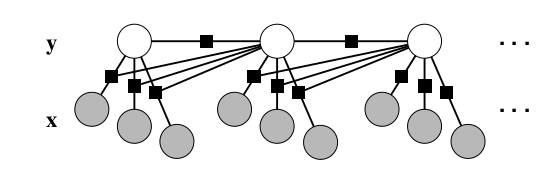
\includegraphics[width=0.7\textwidth]{Bilder/crf-modell-charles-andrew}
\caption{CRF-Modell (die Abbildung ist aus der Arbeit von Charles Sutton \cite{Charles/Andrew:10} entnommen)}
\label{fig:CRF-Modell}
\end{figure}
Die Eckpunkte dieses Graphs beschreiben dabei die Werte, die ,,vorhersagt`` werden müssen (Vektor $Y$ - die Labels, die sagen, ob das Wort eine Entität ist) \textbf{und} die Wörter, für die Labels bestimmt werden müssen (Vektor $X$)\cite{lafferty2001conditional}.

Das CRF-Algorithmus zeigt folgende Vor- und Nachteile auf:
\begin{itemize}
\item Vorteile:
\begin{itemize}
\item Relativ schnelles Trainieren von Modellen\cite{sha2003shallow}, besonders im Vergleich zu SVM.
\item Relativ niedrige Fehlerraten (im Vergleich zu SVM sind die aber doch größer).
\item Die Features müssen nicht unbedingt binär sein, wie es bei ME der Fall ist.
\end{itemize}
\item Nachteile:
\begin{itemize}
\item Die Implementierung von einem CRF-basiertem NER-Extraktor kann komplizierter als die von anderen Algorithmen sein.
\end{itemize}
\end{itemize}

\subsection{Maximum Entropy based NER} \label{sec:MITIEGRUND}
%Was ist ME NER? Wo wird er verwendet? Welche Vor- und Nachteile hat dieser Einsatz im Vergleich zum CRF?
\paragraph{}
Dieses Framework wurde in der Arbeit von Andrew Borthwick\cite{borthwick1999maximum} vorgestellt. ME-Framework operiert grundlegend mit folgenden Begriffen:
\begin{enumerate}
\item \textit{Zukunft} (In \cite{borthwick1999maximum} ,,Futures`` genannt) - Eine Menge von Möglichen Ausgaben (Klassifizierungen von möglichen Entitäten) des Algorithmus.
\item \textit{Historie} - diese Bezeichnung könnte verwirrend wirken, da dieser Begriff eigentlich die Umgebung eines Wortes beschreibt (so eine Art vom Fenster, wo das Wort, das analysiert werden muss, in der Mitte steht).
\item \textit{Features} - wie bei anderen Algorithmen beschreibt dieser Begriff ein Vektor von Eigenschaften eines Wortes.
\end{enumerate}
Ähnlich wie bei CRF wird es versucht die Wahrscheinlichkeit $P(Future|Historie)$, deren Kalkulation in der Formel \ref{eq:meeq} beschrieben ist, zu maximieren. 

Ein gravierender Unterschied zum CRF besteht daran, dass in der ,,üblichen`` Implementierung dieses Algorithmus nur binäre Features\cite{berger1996maximum} $g(w,u)$, deren Form in der Formel \ref{eq:binfeat} beschrieben ist, im Kauf genommen werden können. 

\begin{equation} \label{eq:binfeat}
g(wort, umgebung) = 
\begin{cases}
1  & \text{wenn das Token das untersuchte Eigenschaft besitzt} \\
0 & \text{ansonsten} 
\end{cases}
\end{equation}

\begin{equation} \label{eq:meeq}
p(f|h) = \frac{1}{Z(h)}\prod \alpha_i^{g_i(f,h)}
\end{equation}
Das Wert $\alpha_i$ definiert im ME-Algorithmus das Gewicht einer Eigenschaft. Die Funktion $Z(h)$ ist dabei eine Normalisierungsfunktion und spielt dieselbe Rolle wie $Z(x)$ in der Formel \ref{eq:zeteq}, und ist wie folgt definiert:

\begin{equation} \label{eq:zeteqme}
Z(h) = \sum_f \prod_i \alpha_i^{g_i(f,h)}
\end{equation}

Wie es schon erwähnt wurde, hat ME ein gravierender Nachteil, und zwar dass es nur binäre Eigenschaften verwendet werden können. Allerdings ist ein ME-Modell schneller als CRF, besonders was Training angeht, und ist auch leichter zu implementieren, deswegen findet auch dieses Algorithmus sein Platz in heutigen NER-Systemen wie OpenNLP\footnote{\url{http://opennlp.apache.org/}}.

\subsection{SVM}
\paragraph{}
Support Vector Machines (oder Stützvektormaschine) ist eine Methode zur Klassifizierung von Daten, deren Grundidee\cite{meyer2014support} auf der Abbildung \ref{fig:SVM-INTRO} graphisch dargestellt ist. 

\begin{figure}
\centering
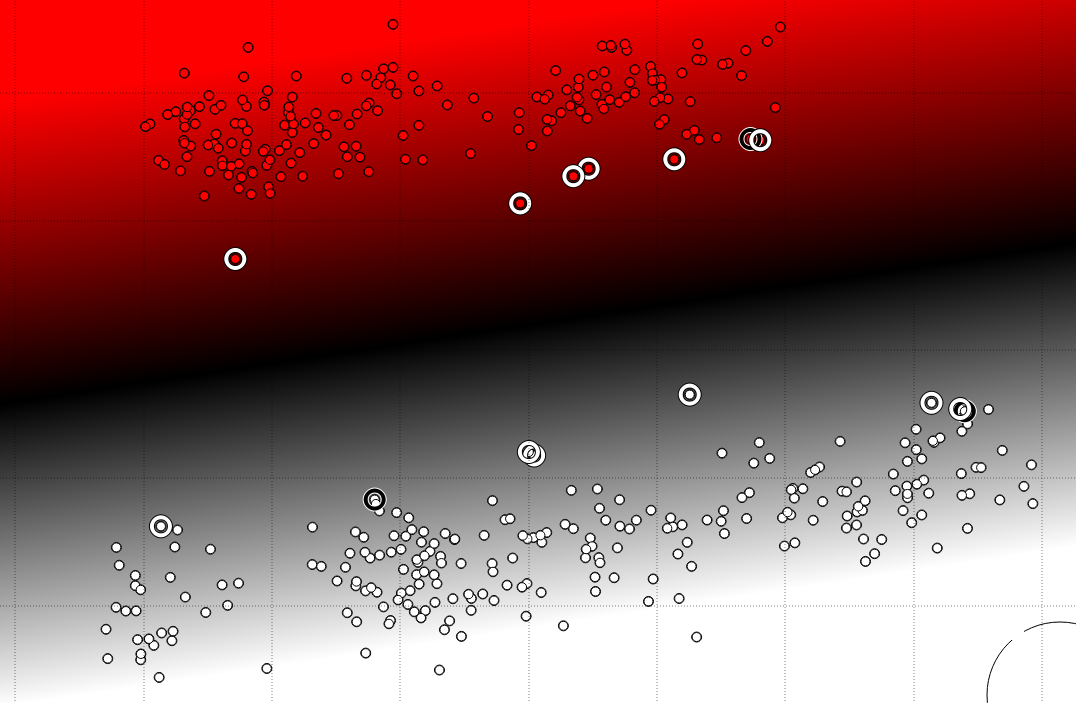
\includegraphics[width=\textwidth,angle=90]{Bilder/svm-intro.png}
\caption{''Die Klassifizierung mithilfe von Stützvektoren''}
\label{fig:SVM-INTRO}
\end{figure}

Der SVM-Klassifikator versucht, für eine Menge von \textbf{linear trennbaren} Punkten in einem Vektorraum eine Hyperebene zu finden, die die Punkte in zwei Klassen aufteilt, und zwar so, dass der Abstand zwischen dieser Trennfläche und den Randpunkten möglichst maximal bleibt.

\paragraph{}
Damit so eine Hyperebene aufgebaut werden könnte, ist es wichtig, dass die Datenpunkte linear trennbar sind. Wenn das SVM-Algorithmus direkt auf nicht linear trennbare Daten angewendet wird, wird die resultierende Trennebene falsch aufgebaut, was auf der Abbildung \ref{fig:SVM-NONLINEAR-ISSUE} zu sehen ist. 

Allerdings sind meiste Daten, mit denen man in der realen Welt arbeiten muss, nicht linear trennbar, und damit kann das SVM-Algorithmus nicht in seiner ursprünglichen Form verwendet werden. Allerdings gibt es eine Möglichkeit, mit einer Erweiterung von SVM-Einsatz auch nicht linear trennbare Daten zu klassifizieren. Dazu muss das ursprüngliche Eigenschaftensraum auf ein Raum höherer Dimension abgebildet werden, und zwar so, dass die Datenpunkte in neuem Raum linear trennbar wären\cite{Hearst:98}.

Das Verfahren, das solche Abbildung ermöglicht, heißt ,,Kernel``, und ist in der Arbeit von Hsu\cite{hsu2003practical} beschrieben. Ein Kern ist eine Funktion 
$K(x_i,x_j) = \phi(x_i)^T \phi(x_j)$, die den Punkt im ursprünglichen Raum $R^{n_1}$ auf ein Punkt im Raum $R^{n_2}$ abbildet, so dass $n_1 < n_2$ ist. In der Praxis sind laut Hsu\cite{hsu2003practical} folgende Kernfunktionen etabliert:
\begin{enumerate}
\item Lineares Kern: $K(x_i,x_j) = x_i^T x_j$
\item Polynominales Kern: $K(x_i,x_j) = (\gamma x_i^T x_j + r)^d, \gamma > 0$
\item Radiale Basisfunktion (RBF): $K(x_i,x_j) = exp(-\gamma \Vert x_i - x_j \Vert^2), \gamma > 0$
\item Sigmoid : $K(x_i,x_j) = tanh(\gamma x_i^T x_j + r)$
\end{enumerate}
Die Variablen $\gamma$, $r$ und $d$ sind benutzerdefinierte Kernelparameter.

\begin{figure}
\centering
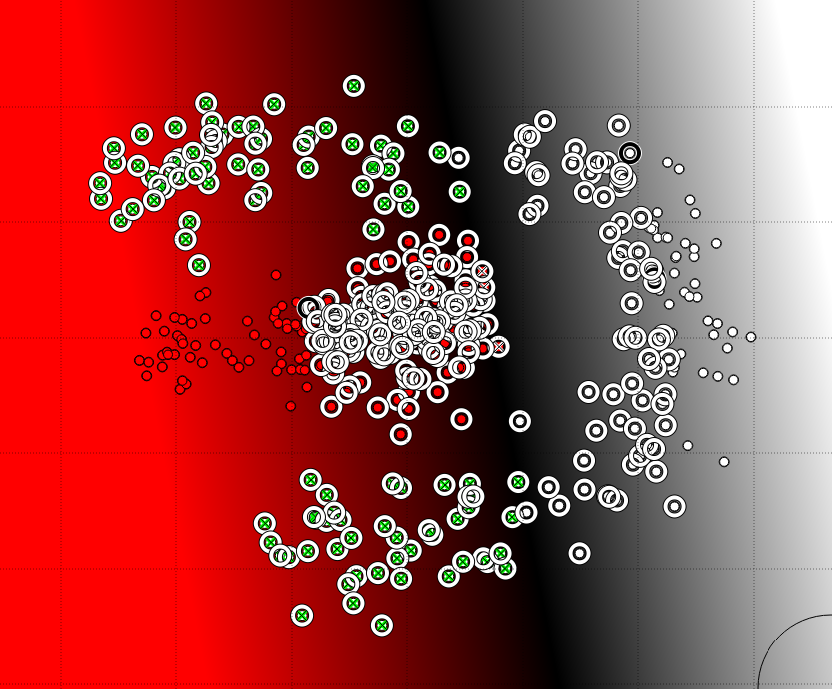
\includegraphics[width=\textwidth,angle=90]{Bilder/svm-nonlinear-issue.png}
\caption{''SVM Algorithmus angewandt auf nicht linear trennbare Daten''}
\label{fig:SVM-NONLINEAR-ISSUE}
\end{figure}

\begin{figure}
\centering
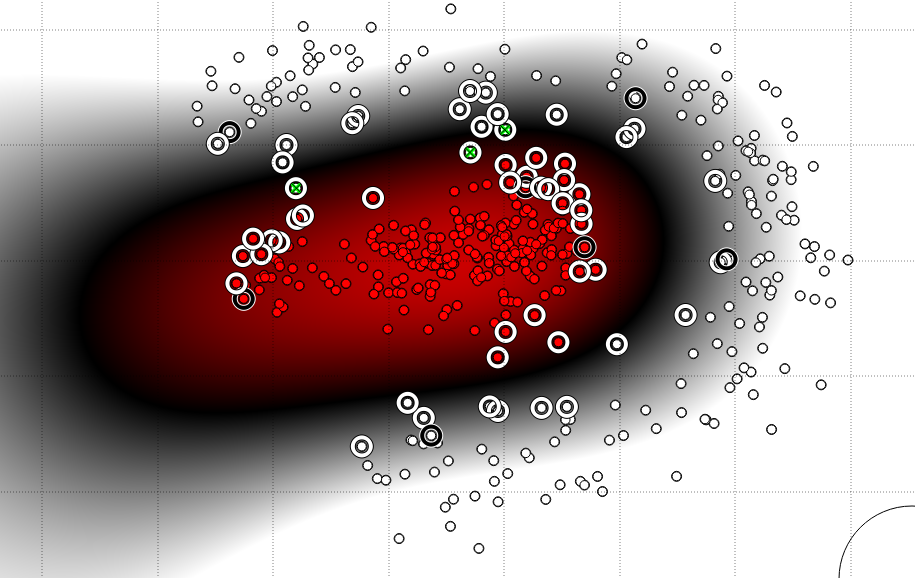
\includegraphics[width=\textwidth,angle=90]{Bilder/svm-nonlinear-rbf.png}
\caption{''SVM-Algorithmus mit einem RBF-Kern angewandt auf nicht linear trennbare Daten''}
\label{fig:SVM-NONLINEAR-ISSUE}
\end{figure}

\paragraph{}
%Und wie kann man SVMs in NEr einsetzen?
Der Einsatz von Stützvektoren für Extraktion von Entitäten ist in der Arbeit von Kazama\cite{kazama2002tuning} beschrieben. Obwohl es in dieser Arbeit um Extraktion von Entitäten aus englischsprachigen medizinischen Texten geht, kann dasselbe Prinzip auch auf deutsche Texte angewendet werden, wenn man das richtige Korpus für Training zur Verfügung stellt. Um SVMs für Extraktion von Entitäten einsetzen zu können, muss noch eine Erweiterung zum ursprünglichen Algorithmus gemacht werden, zusätzlich zum Kerneleinsatz - Stützvektoren können generell zwischen zwei Klassen von Objekten unterscheiden (ein Stützvektoreinsatz kann sagen, ob das Objekt der Klasse $C_a$ oder der Klasse $C_b$ gehört), und bei Entitäten gibt es mehr als zwei Klassen. Um diese Beschränkung umzugehen, wird SVM-Algorithmus auf eine der folgenden Arten und Weisen erweitert:

\begin{itemize}
\item Für jede mögliche Entitätsklasse wird ein SVM aufgebaut, der entscheidet, ob das Token der Klasse $C_a$ oder dem Rest der Klassen gehört.
\item Für jede Paar $(C_a, C_b)$ von möglichen Entitätstypen wird ein SVM erzeugt, der feststellen muss, ob das Wort den Typ $C_a$ oder $C_b$ hat. Die Klasse, die von der Mehrheit von SVMs gewählt wurde, gewinnt.
\end{itemize}

\paragraph{}
Vorteile des SVM-Einsatzes anderen Methoden gegenüber\cite{joachims1998text}:
\begin{itemize}
\item SVMs eignen sich gut für die Bearbeitung von langen Featuresvektoren, was bei Klassifizierung von Wörtern ein großer Vorteil ist.
\item Dieses Algorithmus funktioniert mehr oder weniger gleich auf allen Domänen von Texten.
\item Es ist üblicherweise kein Tuning von Traininsparametern notwendig.
\end{itemize}

Nachteile von SVMs anderen Einsätzen gegenüber:
\begin{itemize}
\item Relativ langsamer Trainingsvorgang - bei größeren Trainigskorpora kann die Erstellung eines Modells bis auf mehrere Tagen in Anspruch nehmen.
\item Anforderungen zur Größe des Arbeitsspeichers sind üblich auch höher als bei anderen Algorithmen.
\end{itemize}

\section{Trainingskorpora} \label{sec:trcorpora}
Jedes im Rahmen dieser Arbeit betrachtetes Algorithmus braucht ein vortrainiertes Modell, um Entitäten aus einem Text extrahieren zu können. Manchmal können zwar schon fertige Modelle verwendet werden, die schon vorher trainiert wurden, aber wenn es kein solches Modell verfügbar ist, muss der Entwickler ein eigenes trainieren.

Um ein Modell trainieren zu können, braucht man ein Textkorpus. Korpus ist eine Sammlung von Texten, die entweder von Linguisten (manuell annotierete Korpora) oder automatisch (maschinell erzeugte Korpora) mit Annotationen versehen wurden. Die Annotationen können im Prinzip beliebig sein (z.B. POS-Tags sind auch Annotationen), aber im Rahmen der Erkennung von Entitäten braucht man ein Korpus, wo die Wörter, die Entitäten darstellen, markiert sind \cite{naf2006korpuslinguistik}.

Ein Beispiel für ein von Linguisten vorbereitetes Korpus wäre auf Zeitungen und Zeitschriften aufgebautes CoNLL \cite{tjong2003introduction}. Die Daten, die im Rahmen der verlinkten Arbeit gesammelt wurden, haben folgende Vorteile:
\begin{itemize}
\item Da dieses Korpus auf Zeitschriften aufgebaut ist, weisen die Daten relativ gute Qualität auf, vor allem im Bezug auf Schreibfehler.
\item Das in diesem Korpus verwendetes Datenformat ist ein Industriestandard und ist deswegen bereits in vielen Bibliotheken für Analyse von natürlichsprachlichen Texten implementiert. 
\item Ein Korpus für deutsche Sprache ist auch verfügbar, was die Daten nützlich für diese Masterarbeit machen könnte.
\end{itemize}
Leider konnten diese Daten im Rahmen dieser Arbeit nicht verwendet werden, da die öffentlich nicht verfügbar sind, und nur gegen Aufpreis zur Verfügung gestellt werden können. In der Sektion \ref{sec:extraktimpl} des Kapitels ,,Implementierung`` wird es deswegen auf Alternativlösungen zugegriffen.

Eine Alternative zu den auf Basis von Zeitungen aufgebauten Korpora wären die webbasierte Korpora\cite{liu2006web}. Im Vergleich zu den auf Zeitschriften basierten Korpora, weisen die aus Web extrahierte Daten größere Varianz auf, und wären deswegen für generische Domäne nützlicher sein können. Es muss aber gleichzeitig beachtet werden, dass die aus Web extrahierte Daten größere Fehlerraten aufweisen können, besonders im Bezug auf Grammatik. Ein Beispiel für ein webbasiertes Korpus wäre DeWaC\cite{baroni2009wacky}.

Zusätzlich zu manuell erstellten Korpora könnte ein Korpus auch automatisch erstellt werden, wie es z.B. für POS-Annotationen in der Arbeit von Marcus\cite{marcus1993building} gemacht wurde. In der Sektion \ref{subsec:decor} des Kapitels ,,Implementierung`` wird die Erstellung eines Korpus für Entitätsextraktion auf Basis von aus Wikipedia extrahierten Daten näher beschrieben.

Beim Training eines NER-Modells auf einem Korpus muss außerdem folgendes im Kauf genommen werden: bei vielen frei verfügbaren Korpora sind die Klassen von Entitäten nicht explizit eingegeben - die Entitäten sind in vielen Datensätzen zwar annotiert, aber weitere Angaben zum Typ der Entität werden nicht gemacht. Deswegen kann ein NER-Modell den Unterschied zwischen verschiedenen Klassen von Entitäten öfters nicht lernen, was dazu führt, dass die entsprechende Klassen nachdem die Entitäten aus einem Text extrahiert wurden aus einer Datenbank geholt werden müssen, falls die Daten vorhanden sind.

\section{Wissendatenbanke} \label{sec:wiss}
%Was sind Wissendatenbanke? Wieso brauchen wir die in unserer Arbeit? Wie sucht man nach Entitäten in einer Wissendatenbank? Kurze Einleitung in SPARQL+RDF.
\paragraph{}
Um die extrahierte Entitäten mit Ontologien anzureichern, braucht man selbstverständlich eine Datenbank, wo alle Informationen zu den Entitäten gespeichert werden. Solche Datenbanken nennt man ,,Wissendatenbanken`` - eine Datenbank, wo ,,Wissen`` über ein bestimmtes Domain gespeichert werden. Es stellt sich die Frage, warum die ,,Wissendatenbanken`` explizit von den herkömmlichen relationalen Datenbanken getrennt behandelt werden müssen. Welche Besonderheiten weisen Wissendatenbanke auf, die Anwendung von relationalem Datenmodell schwer (beziehungsweise unmöglich) machen?

Aus den verschiedenen Werken über relationale Algebra\cite{meier2013relationale} ist es bekannt, dass relationale Datenbanken ,,fest`` strukturiert sind - die Daten sollen einer vordefinierten Schema (Beschreibung der Datenstruktur) folgen. Jede Änderung von Datenstruktur (das Hinzufügen von neuen Feldern z.B.) führt zu einer Schemaänderung. Es ist allerdings sehr schwer, solche ,,feste`` Schema für Entitäten zu definieren, da:
\begin{itemize}
\item Verschiedene Entitäten können verschiedene Menge von Eigenschaften besitzen - ein geographisches Objekt kann kein Geburtstag haben, eine Person allerdings schon.
\item Sowohl die Klassen als auch die Eigenschaften können sich mit der Zeit ändern - neue Klassen können hinzugefügt und alte Eigenschaften gelöscht werden.
\item Die Entitäten können mithilfe von Links miteinander verbunden sein, und diese Links können zyklisch sein, was auf der Abbildung \ref{fig:cyclent} dargestellt ist. Es ist zwar möglich, zyklische Datenstrukturen mithilfe von relationalen Datenbanken abzubilden versuchen, die Aufbau solcher Datenbank wäre aber zu komplex.
\end{itemize}

\tikzset{main node/.style={circle,fill=blue!20,draw,minimum size=1cm,inner sep=0pt}}
\begin{figure}[ht]
\setbox0\vbox{\small}
\begin{tikzpicture}[->,>=stealth',shorten >=1pt,auto,node distance=2.8cm,
                    semithick]
\node[main node] (Deutschland) {Deutschland};                      
\node[main node] (Merkel) [above = 3cm of Deutschland] {Angela Merkel};     

\path (Deutschland) edge [bend left] node {Bundeskanzler} (Merkel)
      (Merkel) edge node {Geboren in} (Deutschland);                
\end{tikzpicture}
\caption{Beispiel von zyklischen Verlinkungen zwischen Entitäten}
\label{fig:cyclent}
\end{figure}
Aber wie können dann ,,Wissen`` über die Entitäten gespeichert werden? Welche Datenbanken und Datenstrukturen können hierfür verwendet werden? Gibt es schon bereits eine Lösung oder muss ein eigenes Konzept entwickelt werden?

Für die Darstellung von Wissen wurde von dem W3-Consortium\cite{klyne2006resource} eine spezielle auf XML basierende Datenstruktur RDF (Resource Description Framework) entworfen, die Speicherung von vage strukturierten Daten ermöglicht, was für die Speicherung von Informationen über Entitäten am besten passt. Dieses Format basiert sich auf gerichteten Graphen (siehe die Abbildung \ref{fig:graph-rdf}) und umfasst folgende Grundbegriffe:
\begin{itemize}
\item Subjekt - die Entität, deren Eigenschaft beschrieben werden muss (z.B. eine Person).
\item Prädikat sagt, welche Eigenschaft der Entität beschrieben wird (z.B. Alter einer Person kann ein Prädikat sein).
\item Objekt - das Wert der Eigenschaft. Dabei kann Objekt eine weitere Entität sein, und eigene Eigenschaften besitzen. 
\end{itemize}
Ein Objekt kann also auch die Rolle eines Subjektes spielen und umgekehrt, was die Speicherung von komplexen Strukturen ermöglicht.

\tikzset{main node/.style={circle,fill=blue!20,draw,minimum size=1cm,inner sep=0pt}}
\begin{figure}[ht]
\setbox0\vbox{\small}
\begin{tikzpicture}[->,>=stealth',shorten >=1pt,auto,node distance=2.8cm,
                    semithick]
\node[main node] (Subjekt) {Subjekt};                      
\node[main node] (Objekt) [above = 3cm of Subjekt] {Objekt};     

\path (Subjekt) edge [bend left] node {Prädikat} (Objekt);             
\end{tikzpicture}
\caption{Grundidee des RDF-Datenformats}
\label{fig:graph-rdf}
\end{figure}

Als Backend für die Speicherung von diesen Graphen wird eine Erweiterung von XML benutzt. Ein Beispiel für eine Entität im RDF/XML-Format ist in der Auflistung \ref{lst:RDFBEISPIEL} zu sehen.

\lstset{language=XML}
\lstinputlisting[captionpos=b,label={lst:RDFBEISPIEL},caption={Beispiel einer Ontologie im RDF-Format}]{Listings/examplerdf.xml}

Nachdem das Format für die Datenspeicherung definiert wurde, muss auch eine Anfragesprache definiert werden, mit deren Hilfe auf Informationen in einer Wissendatenbank zugegriffen werden kann. Es ist natürlich klar, dass es hierfür kein SQL verwendet werden kann, da es mit Graphen, und nicht mit relationalen Datenbanken gearbeitet wird. Für die Abfrage von RDF-Daten wird SPARQL (SPARQL Protocol And RDF Query Language) - verwendet. Diese Sprache wurde genau wie RDF-Datenformat vom W3-Consortium entworfen, und ist in der Arbeit von Quilitz\cite{quilitz2008querying} näher beschrieben.

Am besten kann diese Sprache anhand des auf der Auflistung \ref{lst:SPARQLBEISPIEL} abgebildetes Beispiels erklärt werden.
\lstset{language=SPARQL}
\lstinputlisting[captionpos=b,label={lst:SPARQLBEISPIEL},caption={Beispiel einer SPARQL-Anfrage}]{Listings/sparqlexample.sql}

Wie es schon beschrieben wurde, arbeitet SPARQL mit RDF-Graphen. Obwohl diese Abfrage einer SQL-Anfrage ähnlich ist, darf man beide Sprachen nicht verwechseln, da die mit ganz verschiedenen Datentypen arbeiten. 

Eine typische SPARQL-Anfrage ist wie folgt aufgebaut:
\begin{itemize}
\item Der erste Teil der Anfrage - das Schlüsselwort ,,SELECT`` beschreibt, welche Eigenschaften (oder Prädikate in der Terminologie von RDF) einer Entität aus der Datenbank gelesen werden müssen. In dem Beispiel werden die Prädikaten ,,Fläche`` und ,,Bundesland`` benötigt.
\item Der zweite Teil der Anfrage beschreibt, welche Entitäten ausgewählt werden müssen. Auf den ersten Blick sieht die Konstruktion im WHERE-Teil der Anfrage ziemlich kompliziert aus, aber wenn man sich die Abbildung \ref{fig:graph-rdf} anguckt, dann wird es klar, dass es nur so eine Art von einem Muster angegeben wird, das beschreibt, wie Subjekt, Prädikat und Objekt zusammen aussehen müssen, um in der Liste von Ergebnissen aufzutauchen. Die Anfrage im Beispiel \ref{lst:SPARQLBEISPIEL} sagt, dass alle Entitäten, deren Prädikat ,,rdfs:label`` das Wert ,,Duisburg`` hat, und die  außerdem die Eigenschaften ,,dbo:areaTotal`` und ,,dbo:federalState`` besitzen (deren Werte beliebig sein dürfen), aus der Datenbank ausgelesen werden müssen.
\end{itemize}

Optional können die Ergebnisse auch sortiert werden, mithilfe von der ,,ORDER BY``-Operation. Die Ergebnisse lassen sich außerdem mithilfe von regulären Ausdrücken präziser rausfiltern,

Als Antwort auf eine SPARQL-Anfrage wird üblicherweise ein RDF-Graph geliefert. Ein Beispiel für die Antwort auf vorher eingegebene Anfrage findet man in der Auflistung \ref{lst:SPARQLRESULT}.

\lstset{language=XML}
\lstinputlisting[captionpos=b,label={lst:SPARQLRESULT},caption={Beispiel der Antwort auf eine SPARQL-Anfrage}]{Listings/sparqlresult.xml}

\section{Zwischenfazit}
Nachdem die Grundlagen dieser Arbeit erklärt wurden, können schon folgende Bemerkungen für den Implementierungsschritt erläutert werden:
\begin{itemize}
\item Training eines Modells stellt eine getrennte Aufgabe dar, und wird deswegen gesondert implementiert werden müssen.
\item Da nur wenige Korpora frei verfügbar sind, wird es unter anderem auf automatisch erzeugte Korpora zugegriffen, was die Qualität der Extration beeinflussen wird.
\item Für den Vergleich zwischen verschiedenen Algorithmen sollen verschiedene Backends implementiert werden, die über eine universale Schnittstelle erreichbar werden müssen.
\item Es muss für die Verlinkung von Entitäten nachgedacht werden, wo genau die Daten über die Entitäten gefunden werden können.
\end{itemize}
